%!TEX TS-program = xelatex
\documentclass[]{friggeri-cv}
\usepackage{afterpage}
\usepackage{hyperref}
\usepackage{color}
\usepackage{xcolor}
\hypersetup{
    pdftitle={},
    pdfauthor={},
    pdfsubject={},
    pdfkeywords={},
    colorlinks=false,       % no lik border color
   allbordercolors=white    % white border color for all
}
\addbibresource{bibliography.bib}
\RequirePackage{xcolor}
\definecolor{pblue}{HTML}{0395DE}

\begin{document}
\header{Josué }{Gutiérrez}
      {Ingeniero Informático}
      
% Fake text to add separator      
\fcolorbox{white}{gray}{\parbox{\dimexpr\textwidth-2\fboxsep-2\fboxrule}{%
.....
}}

% In the aside, each new line forces a line break
\begin{aside}
    ~
    ~
    ~
    ~
    ~
  \section{Telefono}
    +34 664 84 31 37
    ~
  \section{e-Mail}
    \href{mailto:contacto@josuegutierrez.es}{contacto@\\josuegutierrez.es}
    ~
  \section{Web \& Git}
    \href{http://www.josuegutierrez.es}{josuegutierrez.es}
    \href{https://github.com/JoxuMac}{github.com/joxumac}
    ~
  \section{Programación}
    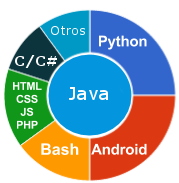
\includegraphics[scale=0.62]{img/programming2.png}
    ~
  \section{S.O.}
    \textbf{MacOS}
\includegraphics[scale=0.40]{img/5stars.png}
    \textbf{Windows}
\includegraphics[scale=0.40]{img/4stars.png}
    \textbf{GNU/Linux}
\includegraphics[scale=0.40]{img/3stars.png}
    ~
  \section{Habilidades}
    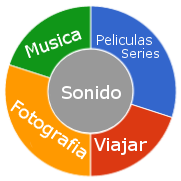
\includegraphics[scale=0.62]{img/personal.png}
    ~
    \section{Idiomas}
    \textbf{Español}
\includegraphics[scale=0.40]{img/5stars.png}
    \textbf{Ingles}
\includegraphics[scale=0.40]{img/3stars.png}
    ~
\end{aside}

\section{Experiencia}
\begin{entrylist}
  \entry
    {09/17 - Ahora}
    {Beca Talentum 2017}
    {Furious Koalas Interactive \& Telefonica}
    {Beneficiario de la Beca Talentum de Telefónica con la empresa Furious Koalas. Equipo de Diseño en el proyecto ARMov de Realidad Aumentada.\\}
  \entry
    {11/17}
    {Voluntariado 1ª Semana Visión por Computador}
    {UCLM, ESI \& VISILAB}
    {Voluntario en la 1ª Semana de la Visión por Computador, Proyecto ref. FCT-1611257, con la colaboración de la Fundación Española para la Ciencia y la Tecnología Ministerio de Economía, Industria y Competitividad, UCLM, Escuela Superior de Informatica y VISILAB.\\}
    \entry
    {05/17}
    {1 Puesto – CTF Hackbits}
    {UCLM, ESI, Hackbits \& Cirebits}
    {Ganador del Primer Puesto en el CTF (Capture de Flag) de ciberseguridad organizado por HackBits.\\}
\end{entrylist}

\section{Educación}
\begin{entrylist}
  \entry
    {2014 - Ahora}
    {Ingeniería Informática}
    {Universidad de Castilla-La Mancha}
    {La Escuela Superior de Informática de CR busca la formación de profesionales capaces de diseñar, gestionar, administrar y mantener sistemas, aplicaciones o productos que permitan la generación, el soporte, el almacenamiento, la transmisión o la organización de la información, con pleno conocimiento de los métodos y técnicas implicados.}\\
\end{entrylist}

\section{Certificaciones}
\begin{entrylist}
  \entry
    {07/2015}
    {CCNA Exploration: Network Fundamentals}
    {Cisco Networking Academy}
    {\emph{\\}}
    \entry
    {04/2015}
    {TOEIC Listening \& Reading}
    {Capman ETS Toeic}
    {\emph{590 Puntos TOEIC.\\}}
    \entry
    {04/2015}
    {Taller Smact Avanttic}
    {\begin{flushright}Universidad Castilla-La Mancha \& \\Avanttic Consultoría Tecnológica S.L.\end{flushright}}
    {\emph{Primera edición de avanttic\_day, como continuación de la jornada de Big Data realizada por la Escuela Superior de Informática.}}
\end{entrylist}
\end{document}
